\chapter{Resultados}

Neste capítulo serão apresentados os resultados preliminares, provenientes dos testes realizados bem como refinamento da ferramenta e seus parâmetros, a sessão 4.1 apresentará os resultados obtidos com o PhotoGuide; na sessão 4.2 os resultados preliminares com o \textit{LSD-SLAM} serão mostrados. A seção 4.3 trará os problemas encontrados.

\section{Resultados com o PhotoGuide}

Primeiramente o aplicativo operou sem usar nenhuma das três formas de filtragem descritas anteriormente, ocasionando num grande número de falsos casamentos, como apresentam as imagens 4.1 e 4.2:

\begin{figure}[!htb]
	\centering
		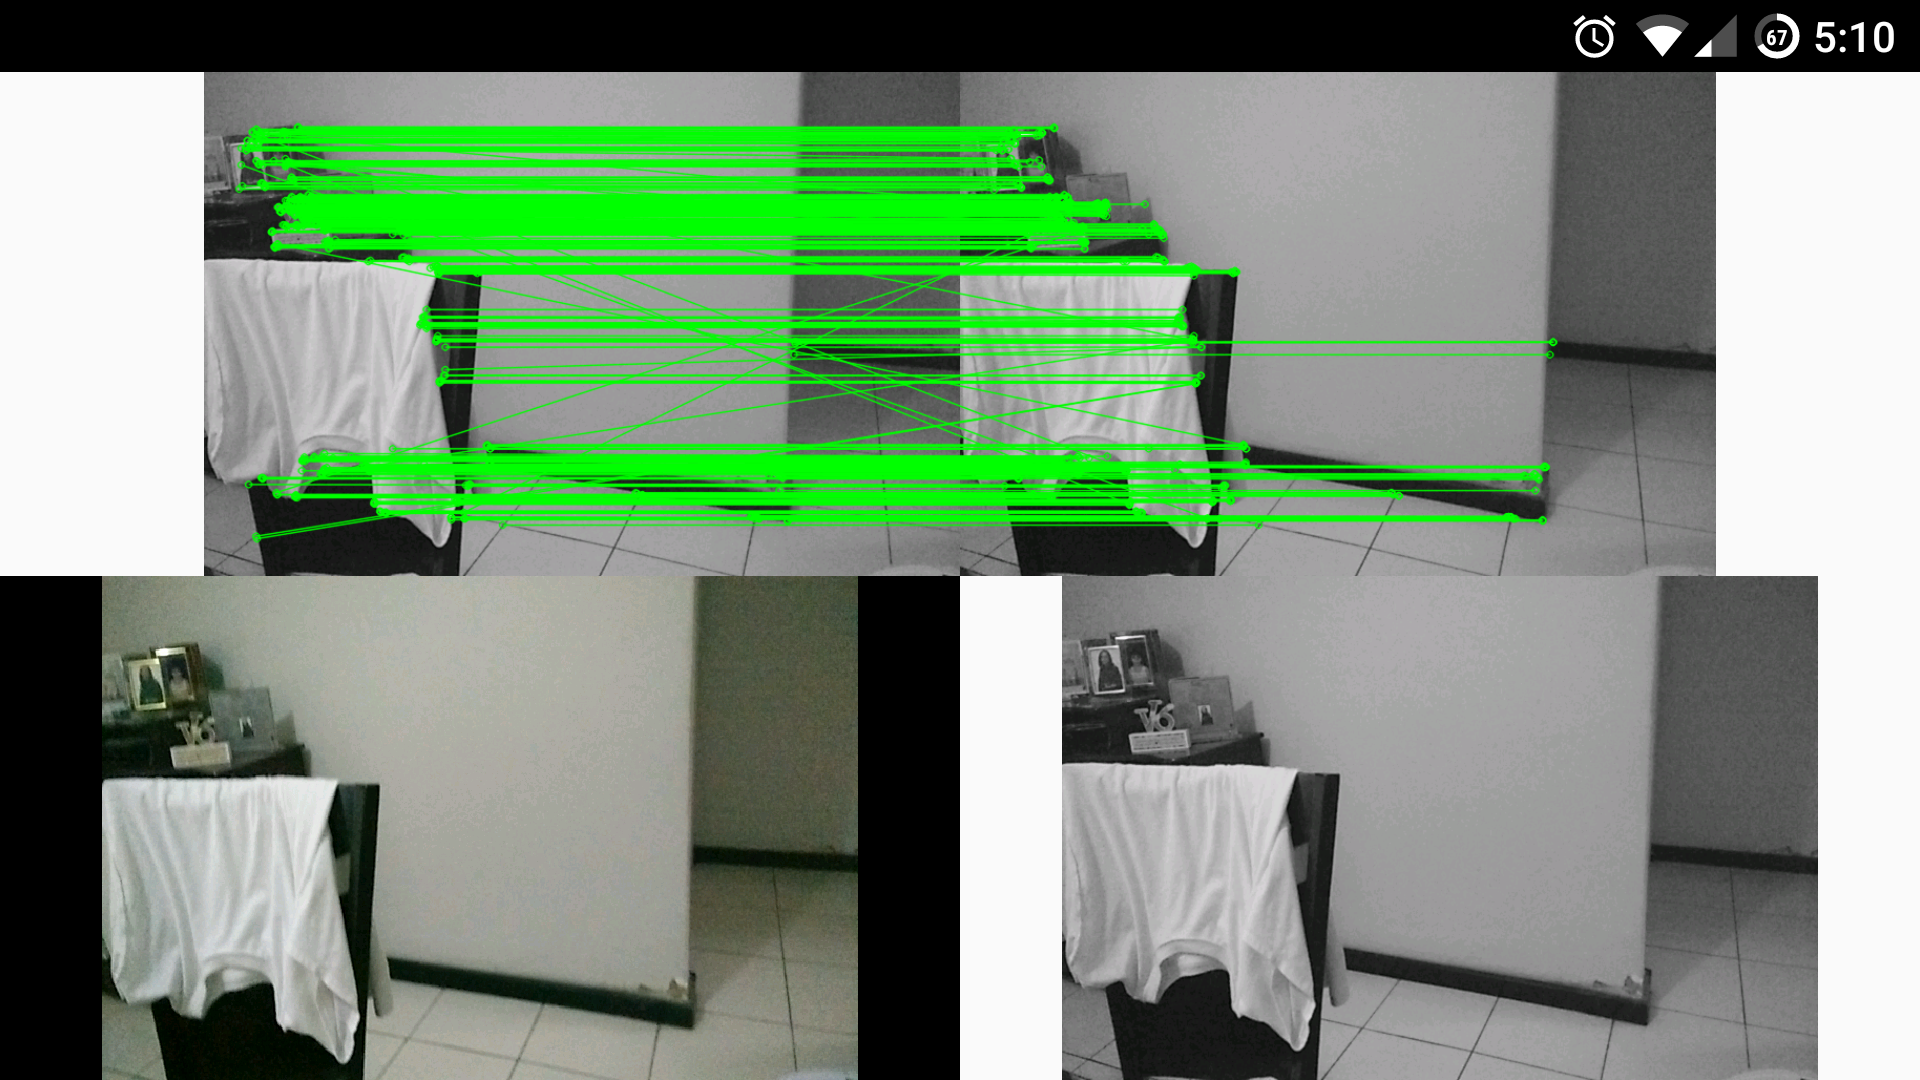
\includegraphics[width= \textwidth]{Imagens/figura4-1.png}
	\caption{Exemplo de execução do PhotoGuide sem nenhuma filtragem de casamentos}
	\label{fig4:1}
\end{figure}

\begin{figure}[!htb]
	\centering
		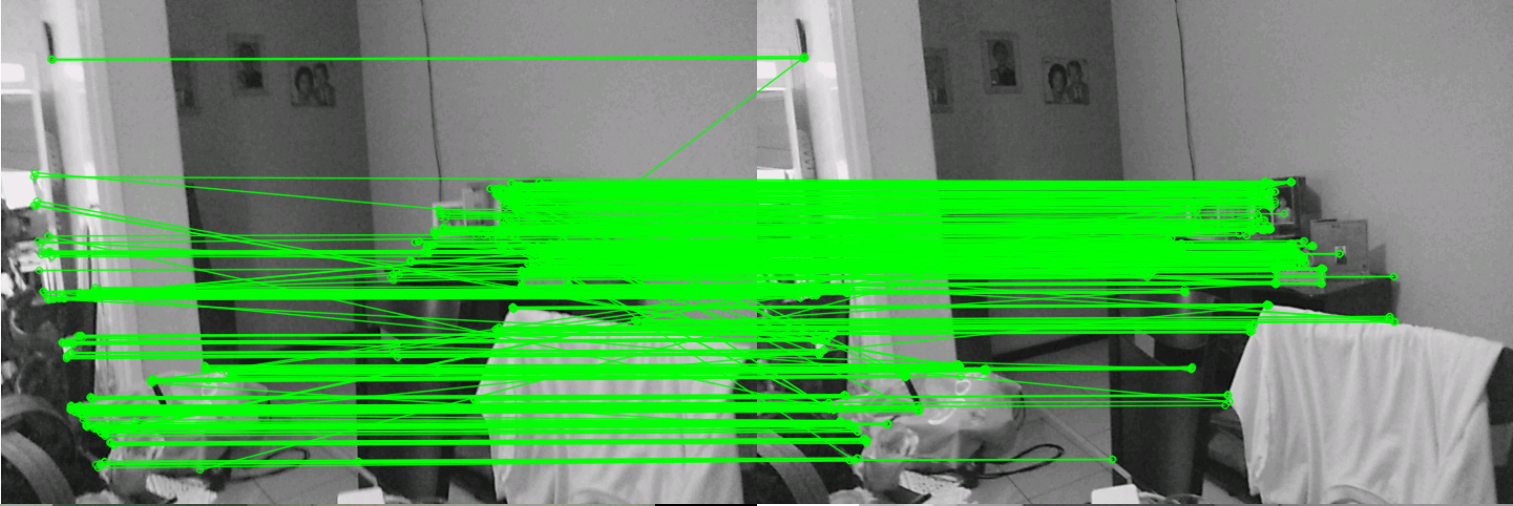
\includegraphics[width= \textwidth]{Imagens/figura4-2.png}
	\caption{Segundo exemplo de execução do PhotoGuide sem nenhuma filtragem de casamentos}
	\label{fig4:2}
\end{figure}

Essa situação é pior quando o ambiente possui partes em vidro, como mesas ou janelas, dificultando ainda mais a casamento de pontos, como mostra a figura 4.3:

\begin{figure}[!htb]
	\centering
		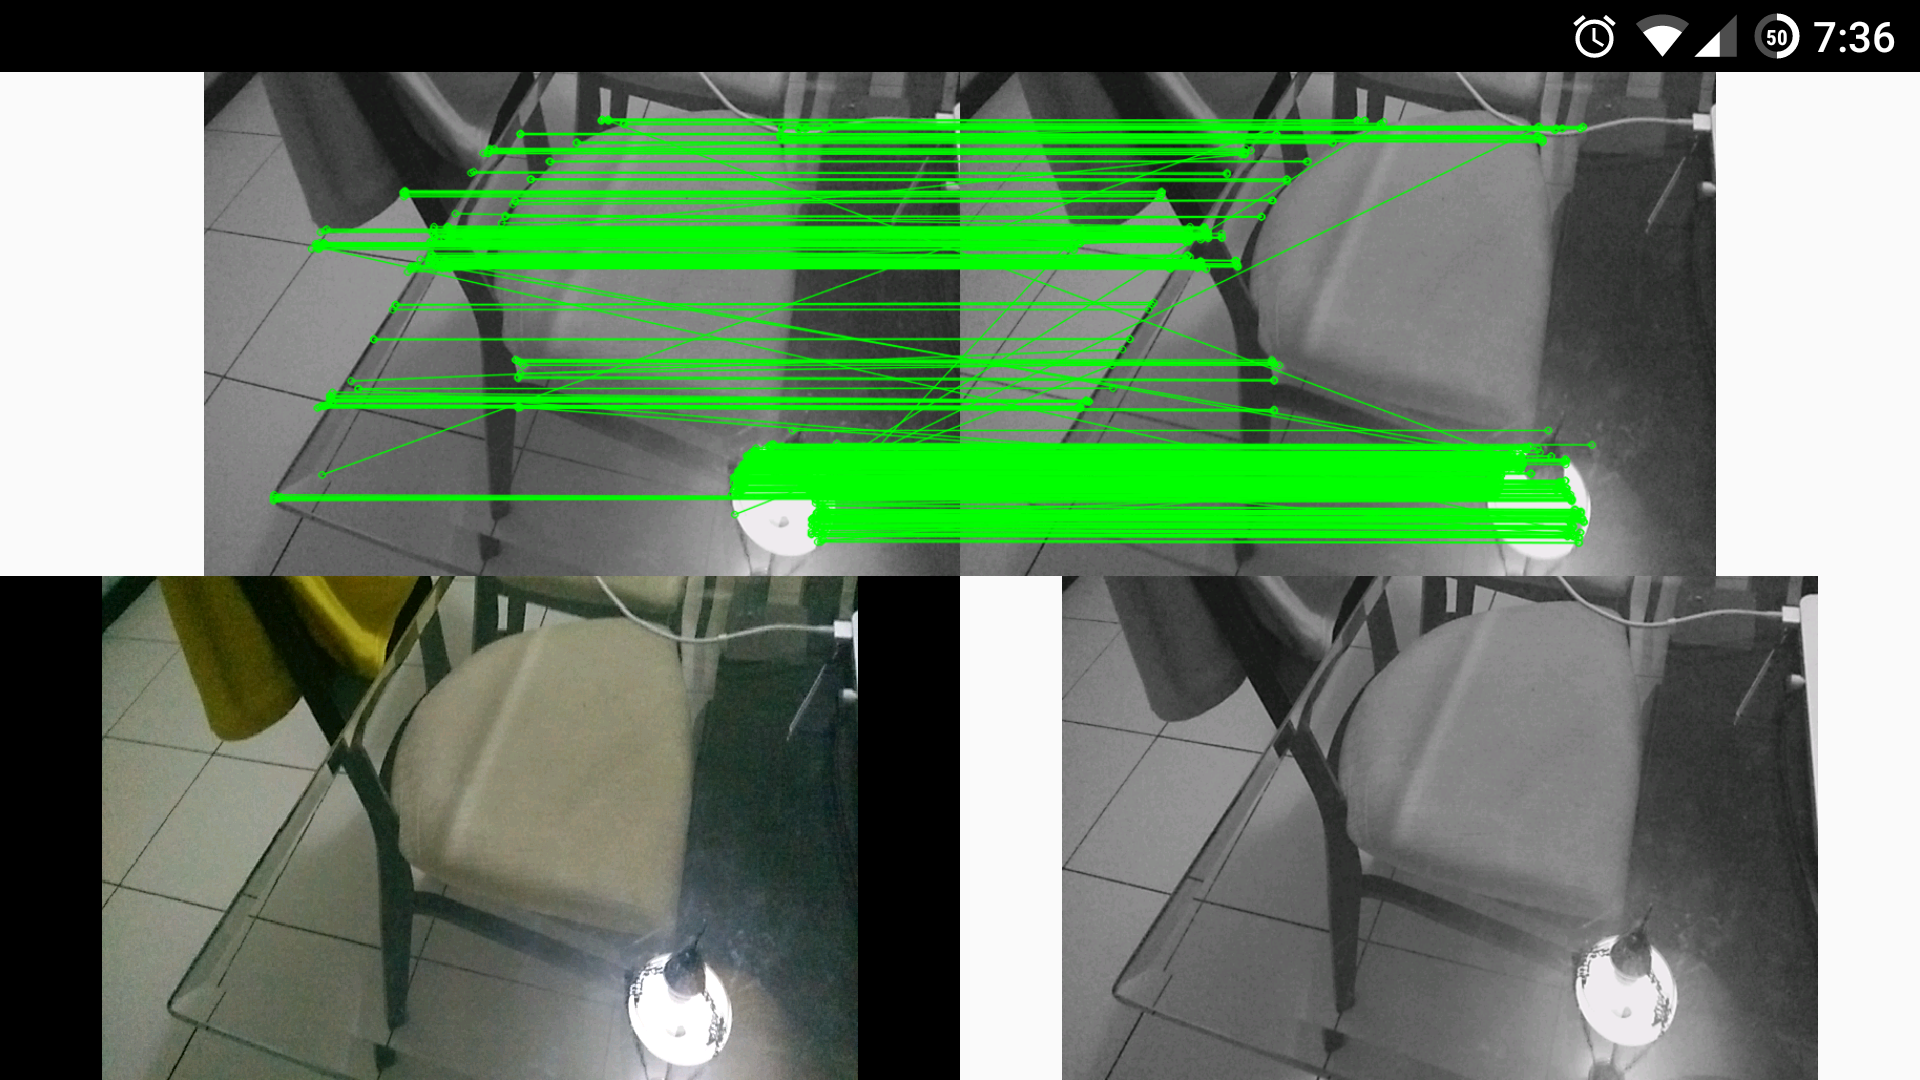
\includegraphics[width= \textwidth]{Imagens/figura4-3.png}
	\caption{Exemplo de execução do PhotoGuide sem nenhuma filtragem de casamentos e com peças em vidro, dificultando os casamentos}
	\label{fig4:3}
\end{figure}

Ao se adicionar os métodos de filtragem explicados na seção 3.1, é possível eliminar diversos casamentos errôneos, como na figura 4.4:

\begin{figure}[!htb]
	\centering
		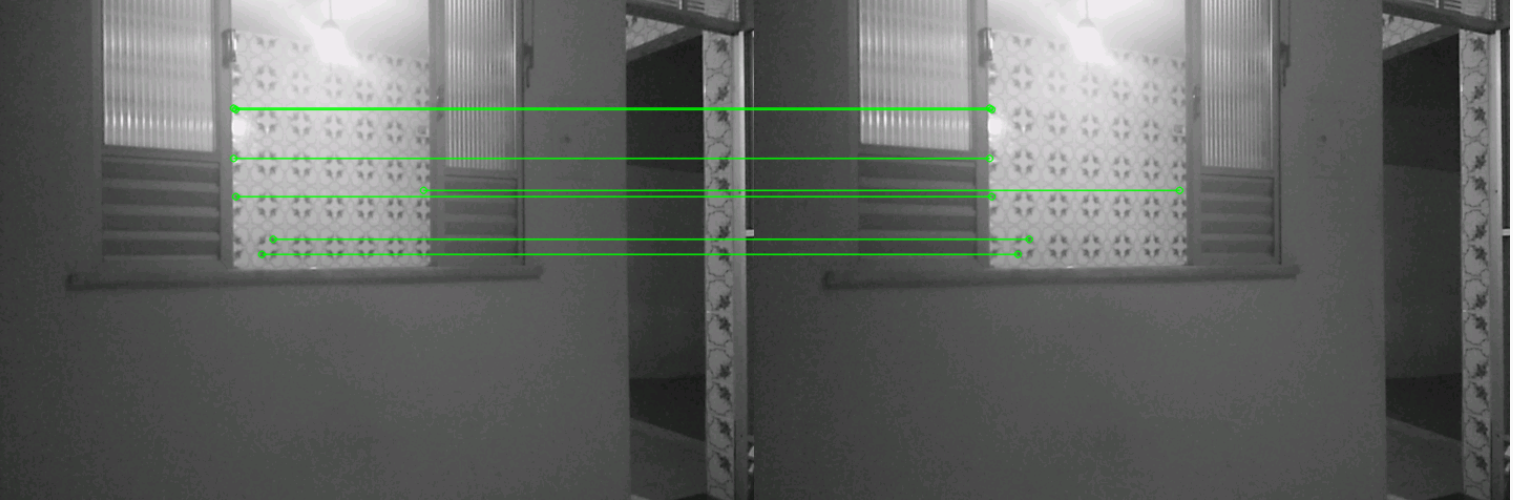
\includegraphics[width= \textwidth]{Imagens/figura3-2E4-4.png}
	\caption{Exemplo da filtragem de casamentos}
	\label{fig4:4}
\end{figure}

Infelizmente, dependendo do ambiente, o número de casamentos pode ser muito pequeno para se tornar significativo para a reconstrução 3D. Foram realizados testes diminuindo a sensibilidade com qual os casamentos eram filtrados, ou a não execução de alguma filtragem, mas ainda eram encontrados falso positivos, sendo necessário todos os métodos de filtragem. 
	Tendo em vista os problemas com o desempenho no aparelho utilizado, bem como problemas com o algoritmo, a continuação do trabalho se deu com a ferramenta \textit{LSD-SLAM}, e a funcionalidade de calibração e exportação de arquivo de calibração do PhotoGuide foi útil para utilizar a calibração de smartphones em testes com o \textit{LSD-SLAM}, bem como a possibilidade de trabalhos futuros onde seja desejado exportar a calibração da câmera ou obter datasets partindo do \textit{smartphone}.
	
\section{Resultados com o \textit{LSD-SLAM}}

O \textit{LSD-SLAM} possui diversos parâmetros que podem auxiliar na visualização e refinamento de como seus algoritmos funcionam. Os testes preliminares foram realizados em um dos laboratórios do DCOMP, mais precisamente, o laboratório de mestrado II, na área externa do prédio e também em um quintal, este último para testar os resultados sob um ambiente com mais texturas e menos homogêneo. As figuras 4.5 a 4.16 mostram as \textit{pointclouds} obtidas e fotografias dos ambientes:

\begin{figure}[!htb]
	\centering
		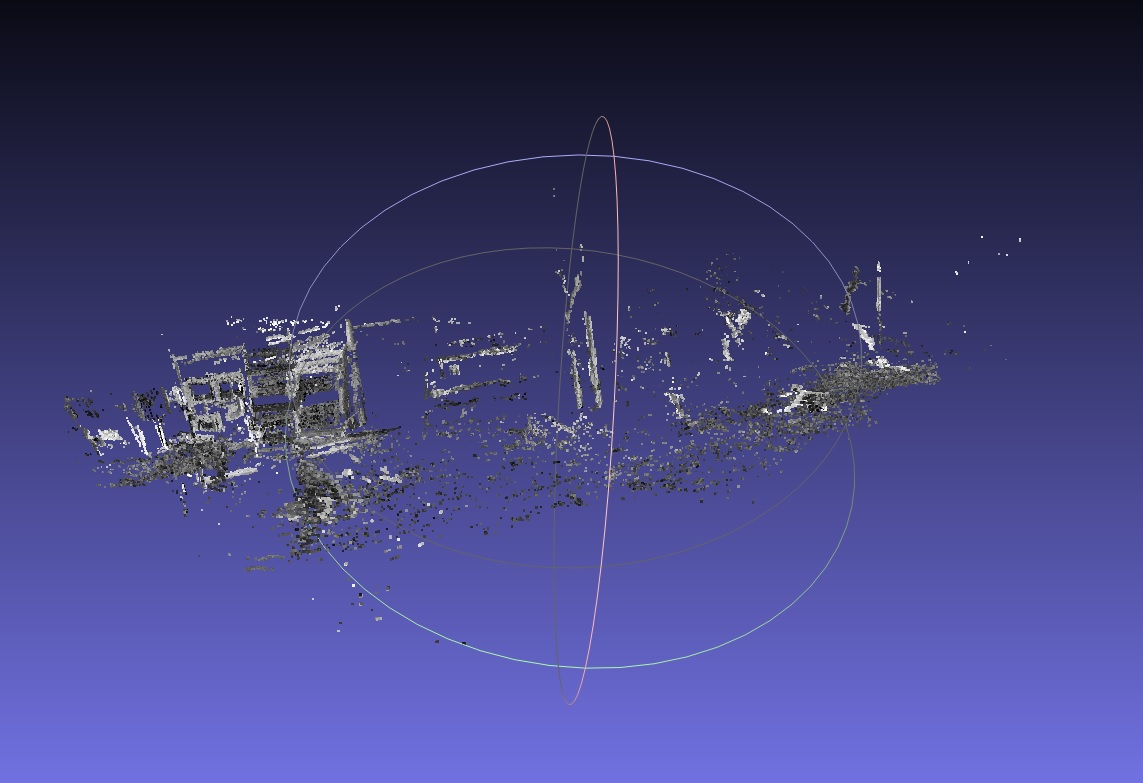
\includegraphics[width= \textwidth]{Imagens/figura4-5.png}
	\caption{Exemplo do \textit{pointcloud} da área externa do DCOMP}
	\label{fig4:5}
\end{figure}

\begin{figure}[!htb]
	\centering
		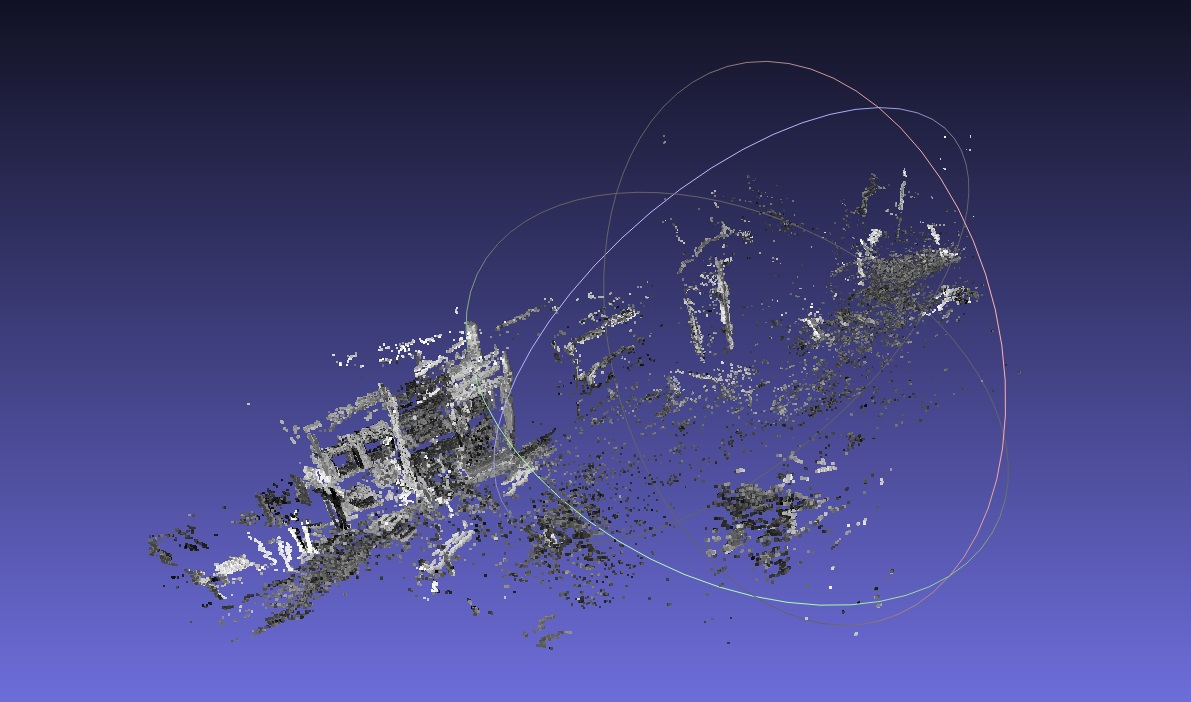
\includegraphics[width= \textwidth]{Imagens/figura4-6.png}
	\caption{Segundo exemplo do \textit{pointcloud} da área externa do DCOMP}
	\label{fig4:6}
\end{figure}

\begin{figure}[!htb]
	\centering
		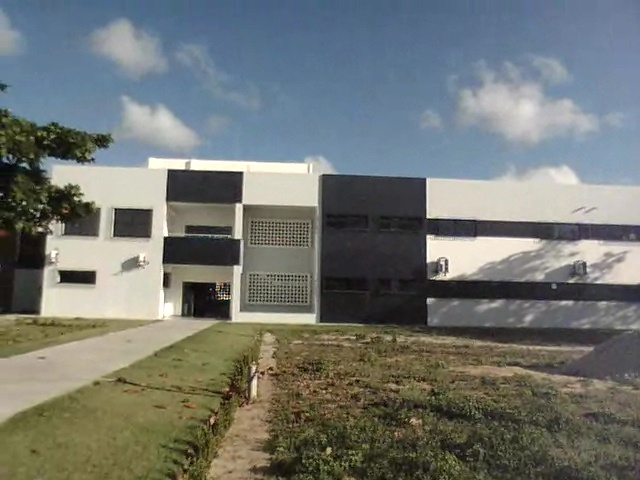
\includegraphics[width= \textwidth]{Imagens/figura4-7.png}
	\caption{Fotografia da área mapeada}
	\label{fig4:7}
\end{figure}

\begin{figure}[!htb]
	\centering
		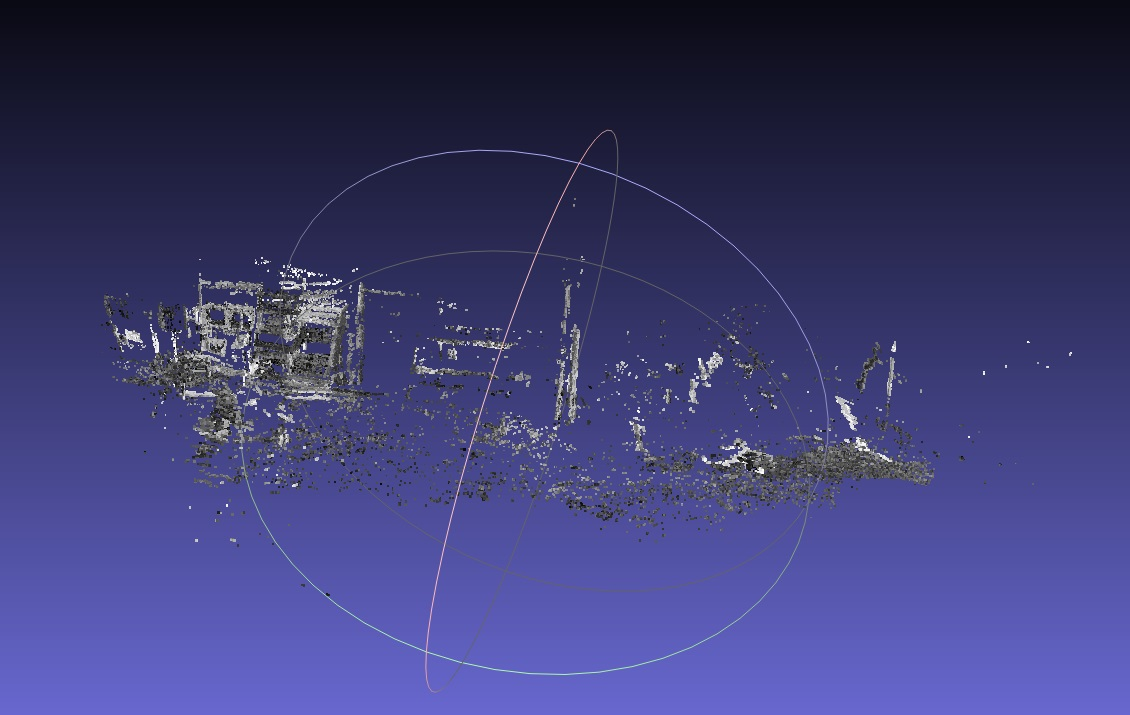
\includegraphics[width= \textwidth]{Imagens/figura4-8.png}
	\caption{Outro \textit{pointcloud} da área externa do DCOMP, sob outro ângulo}
	\label{fig4:8}
\end{figure}

\begin{figure}[!htb]
	\centering
		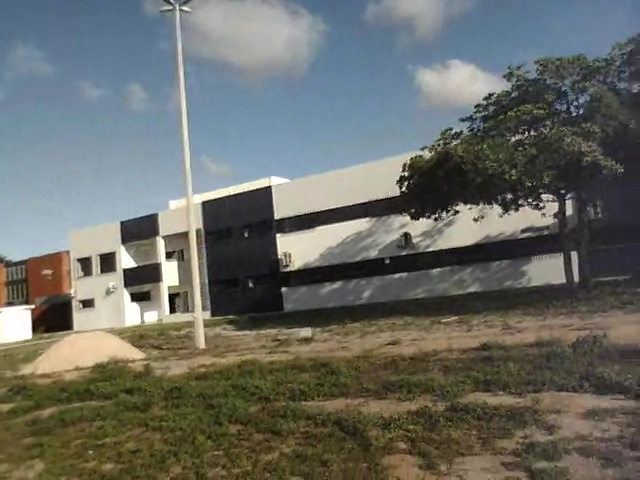
\includegraphics[width= \textwidth]{Imagens/figura4-9.png}
	\caption{\textit{Pointcloud} da figura 4.8}
	\label{fig4:9}
\end{figure}

